\section{実装}
前章で示した二つの手法について,プログラミング言語Pythonを用いて実装を行なった.また両手法についてQUICライブラリaioquic\cite{aioquic}を使用し,手法1についてはICEライブラリaioice\cite{aioice}を使用した.

本稿での実装は\url{https://github.com/kota-yata/2023f-wip}に公開している.

\subsection{手法1の実装}

ICEプロトコルを用いて確立したP2P通信をQUICに再利用する際,通信に使われるソケットを再利用する必要がある.aioice,aioquicともにソケットにライブラリ外部からアクセスする機能は存在しなかったため,aioiceについてはソケットを取り出す処理,aioquicについては接続開始時にソケットを引数として渡す処理を追加し拡張した.

aioiceで通信を確立する際にアドレスペアを交換するための仲介サーバーが必要になるが,これもPythonを用いてWebSocketで通信を行うサーバーを実装した.

\subsection{手法2の実装}
\begin{figure}[h]
  \centering
  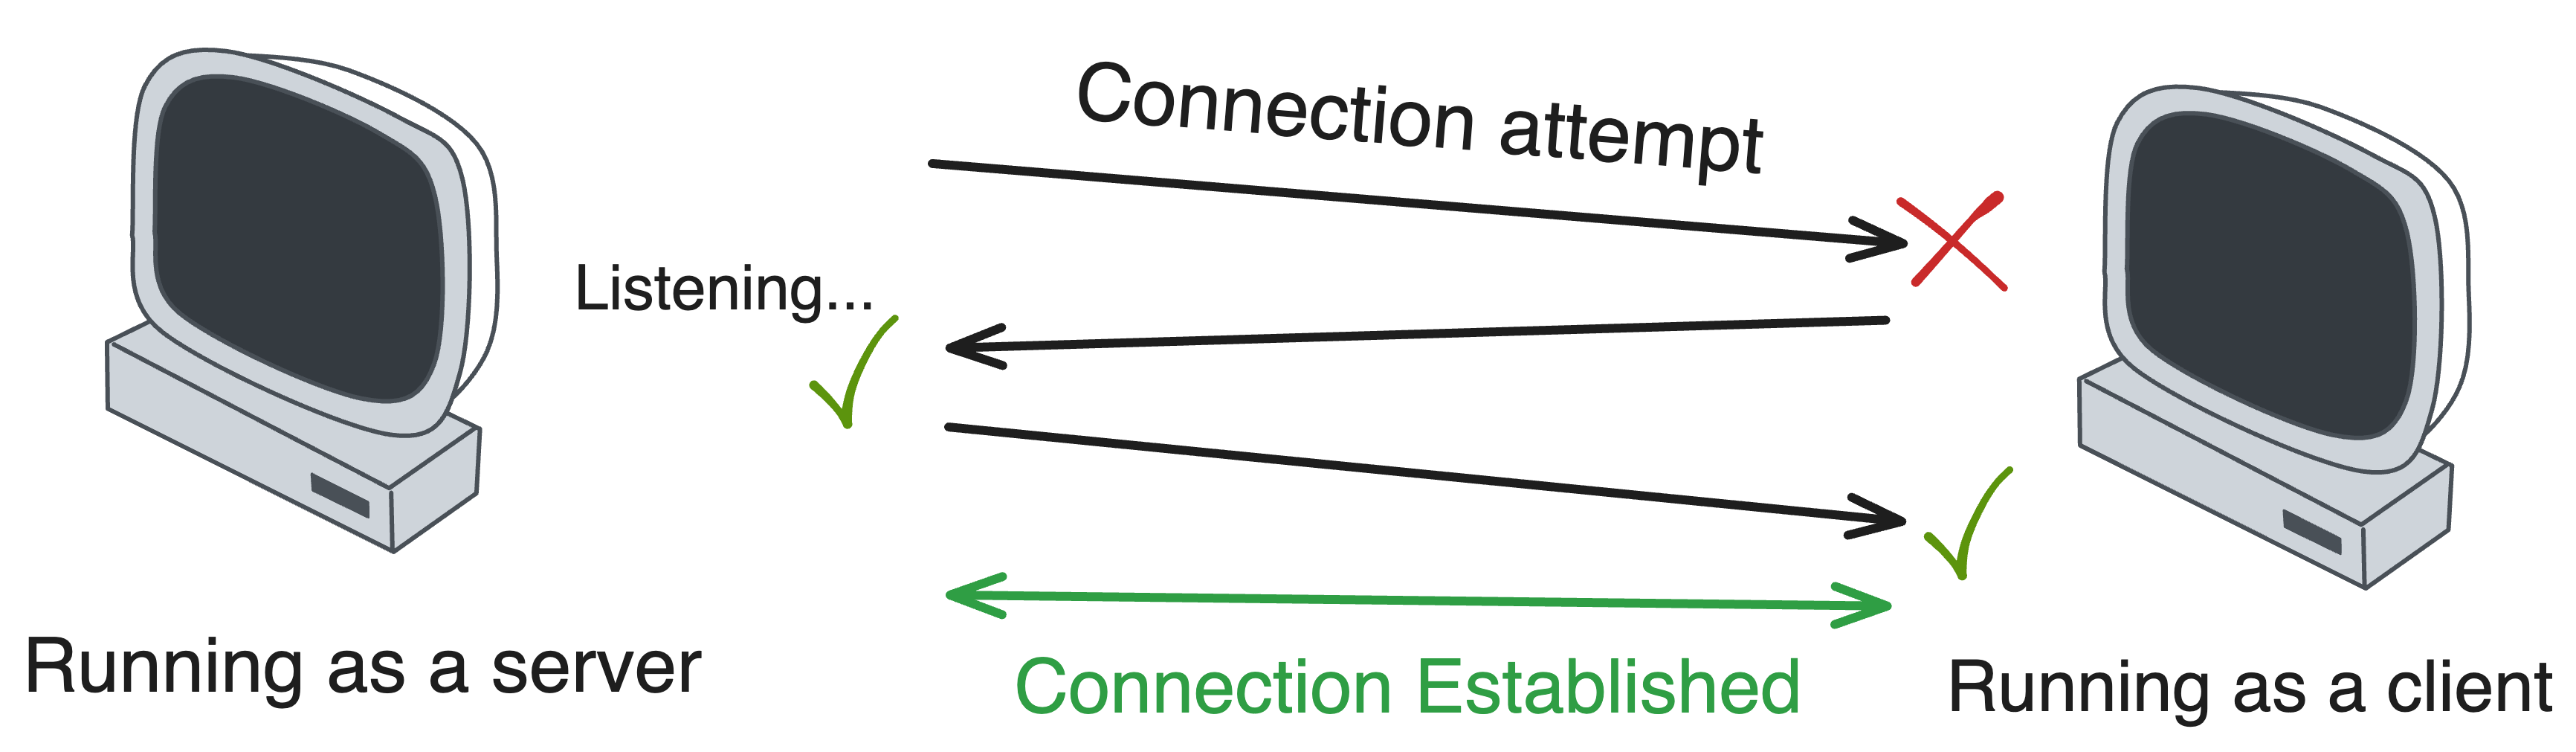
\includegraphics[width=\linewidth]{figs/implement-2.png}
  \caption{QUIC上でのNAT越え}
  \label{fig:impl-2}
\end{figure}
手法2においても,手法1同様にaioquicについて接続開始時にソケットを引数として渡す処理を追加した.また,QUICでは接続開始できるのはクライアント側のみと定義されているが,手法2ではサーバー側からPath Validationフレームを送信する必要があるため,サーバー側からも接続開始できるように拡張をした.

Using QUIC to traverse NATsで提案されているようなICE over QUICの再実装を全て完了することができなかったため,本稿の実装では双方のIPアドレスとポート番号を決め打ちで指定し,Path Validationを送り合ってNAT越えを実現する部分を実装範囲とした.具体的には図~\ref{fig:impl-2}に示すように,片方のピアは接続試行しつつサーバーとして接続を受け付け,もう片方のピアは接続試行を行う.双方から接続試行を行うことで双方のNATデバイスでマッピングが行われ,NAT越えが成立する.本来ICE over QUICが実装できている状態であれば,ICEプロトコルの最初の手順であるSTUNサーバーへの問い合わせの時点でNATマッピングが行われるが,今回はアドレス交換などを省くため図~\ref{fig:impl-2}に示したようなホールパンチングを行った.
